\subsection{Objective}
The Arduino is designed to control a relatively high number of devices. While it is 


a standard code has the following funct() bla bla...

%%%%%%%%%% FLOWCHART%%%%%%%%%%%%%%%%%%%%%%%%%%%%%%%%%%%%%%%%%%%%%%%%%%%%%%%
\newpage
\subsection{Code}

In this section the code written for the robot's controller will be explained. A flowchart diagram of the program is illustrated by Figure \ref{arduinoFlowchart}.\\

As it can be seen, the Arduino first defines all the robot's data, including the motor, servomotor and communication pins. This ensures the microcontroller knows where to send each datum once the user connects to the robot.\\

The program then enters its Loop function. Here it will check if the serial port is available, eg the user has sent a stream of data. Once the port is available, the Read function is called, which stores every byte received into a string to be used later. Once the reading has ended the code checks if it has received a special end-of-line character that signals the end of the data stream. If all the data was retrieved the code moves on to the next function.\\

The Parse function is called upon next. This function's purpose is to break and convert the previously stored string into the corresponding variables needed by each element, taking into account their sizes and types. Hence, it transforms one line of numbers into many parameters such as rotation angle, arm selection or movement direction which will be used by the next function.\\

With the data correctly formatted, the program executes the Process function which is where the "thinking" is done. Here are defined all the rules the robot must follow, such as knowing which claw to close depending on the side chosen by the user but closing both if the symmetry box was checked. It takes the data provided by the previous function and processes them to end up with a structured list of variables ready to be assigned to each element.\\

In the next step the Write function is called. This very simple function goes through the previous list assigning each variable to the corresponding element's assigned pins.\\

Finally, the code clears the initial string to make space for new data, resets the flag informing of the correct retrieval from the serial port and proceeds to the next iteration within the Loop function, restarting the process.\\

	\begin{figure}[H]
			\centering
			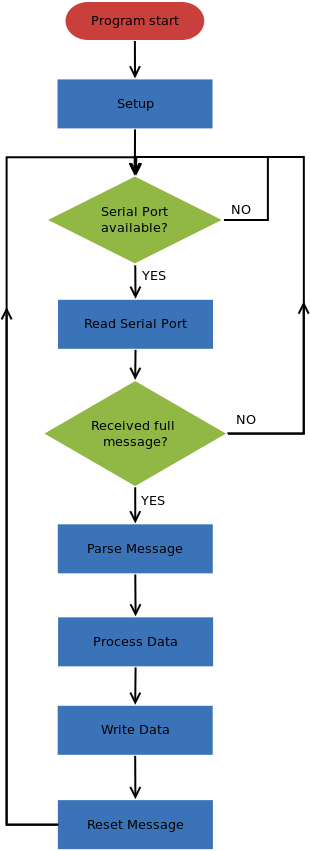
\includegraphics[scale=0.75]{images/Diagrams/arduino2.png}
			\caption{Arduino program flowchart }
			\label{arduinoFlowchart}
	\end{figure}
	\bigskip